\chapter{Results and Analysis} % Main chapter title

\label{Chapter5} % For referencing the chapter elsewhere, use \ref{Chapter5}

%----------------------------------------------------------------------------------------

This chapter presents our experimental results organized around retrieval performance, computational efficiency, embedding space changes, and training dynamics.

\section{Retrieval Performance Results}

Table~\ref{tab:mrr_detailed_thesis} shows all fine-tuning approaches underperform the base model, with MRR@10 degradations ranging from 13.5\% to 32.3\%.

\begin{table}[h]
\centering
\caption{Detailed MRR Performance Comparison}
\label{tab:mrr_detailed_thesis}
\begin{tabular}{lccc}
\toprule
Model & MRR@10 & MRR@100 & \% change in MRR@10 \\
\midrule
Base SBERT & 0.3026 & 0.3144 & — \\
Full FT (Random) & 0.2619 & 0.2723 & -13.5\% \\
Full FT (Hard) & 0.2536 & 0.2632 & -16.2\% \\
LoRA FT (Random) & 0.2557 & 0.2664 & -15.5\% \\
LoRA FT (Hard) & 0.2050 & 0.2149 & -32.3\% \\
\bottomrule
\end{tabular}
\end{table}

\subsection{Performance Pattern Analysis}

Several critical patterns emerge from these results:

\begin{itemize}
\item \textbf{Universal Performance Degradation:} No fine-tuning approach improves upon the base model, contradicting conventional transfer learning expectations
\item \textbf{Hard Negatives Paradox:} Hard negatives consistently perform worse than random negatives, suggesting that semantic similarity-based negative mining may introduce harmful noise to an already optimized model
\item \textbf{LoRA Vulnerability:} LoRA shows greater sensitivity to hard negatives than full fine-tuning, with catastrophic degradation (-32.3\%)
\item \textbf{Scale Mismatch Impact:} Our 1M sample fine-tuning datasets, while substantial, are dwarfed by the base model's 1B sample pre-training
\end{itemize}
\section{Computational Efficiency Analysis}

Table~\ref{tab:inference_detailed_thesis} reveals LoRA models exhibit approximately 2× slower inference despite parameter efficiency, highlighting hidden computational costs in adapter architectures.

\begin{table}[h]
\centering
\caption{Inference Time Analysis (10k Queries)}
\label{tab:inference_detailed_thesis}
\begin{tabular}{lccc}
\toprule
Model & Time (s) & Change from Base & QPS \\
\midrule
Base SBERT & 303.92 & — & 32.9 \\
Full FT (Random) & 324.90 & +6.9\% & 30.8 \\
Full FT (Hard) & 307.48 & +1.2\% & 32.5 \\
LoRA FT (Random) & 574.92 & +89.2\% & 17.4 \\
LoRA FT (Hard) & 598.69 & +97.0\% & 16.7 \\
\bottomrule
\end{tabular}
\end{table}

\section{Embedding Space Analysis}

Figure~\ref{fig:umap_all_thesis} shows UMAP projections revealing progressive embedding space degradation from structured semantic organization in the base model to uniformity in fine-tuned variants.

\begin{figure*}[p]
\centering

% First row: Base and Full FT models
\begin{subfigure}{0.48\textwidth}
\centering
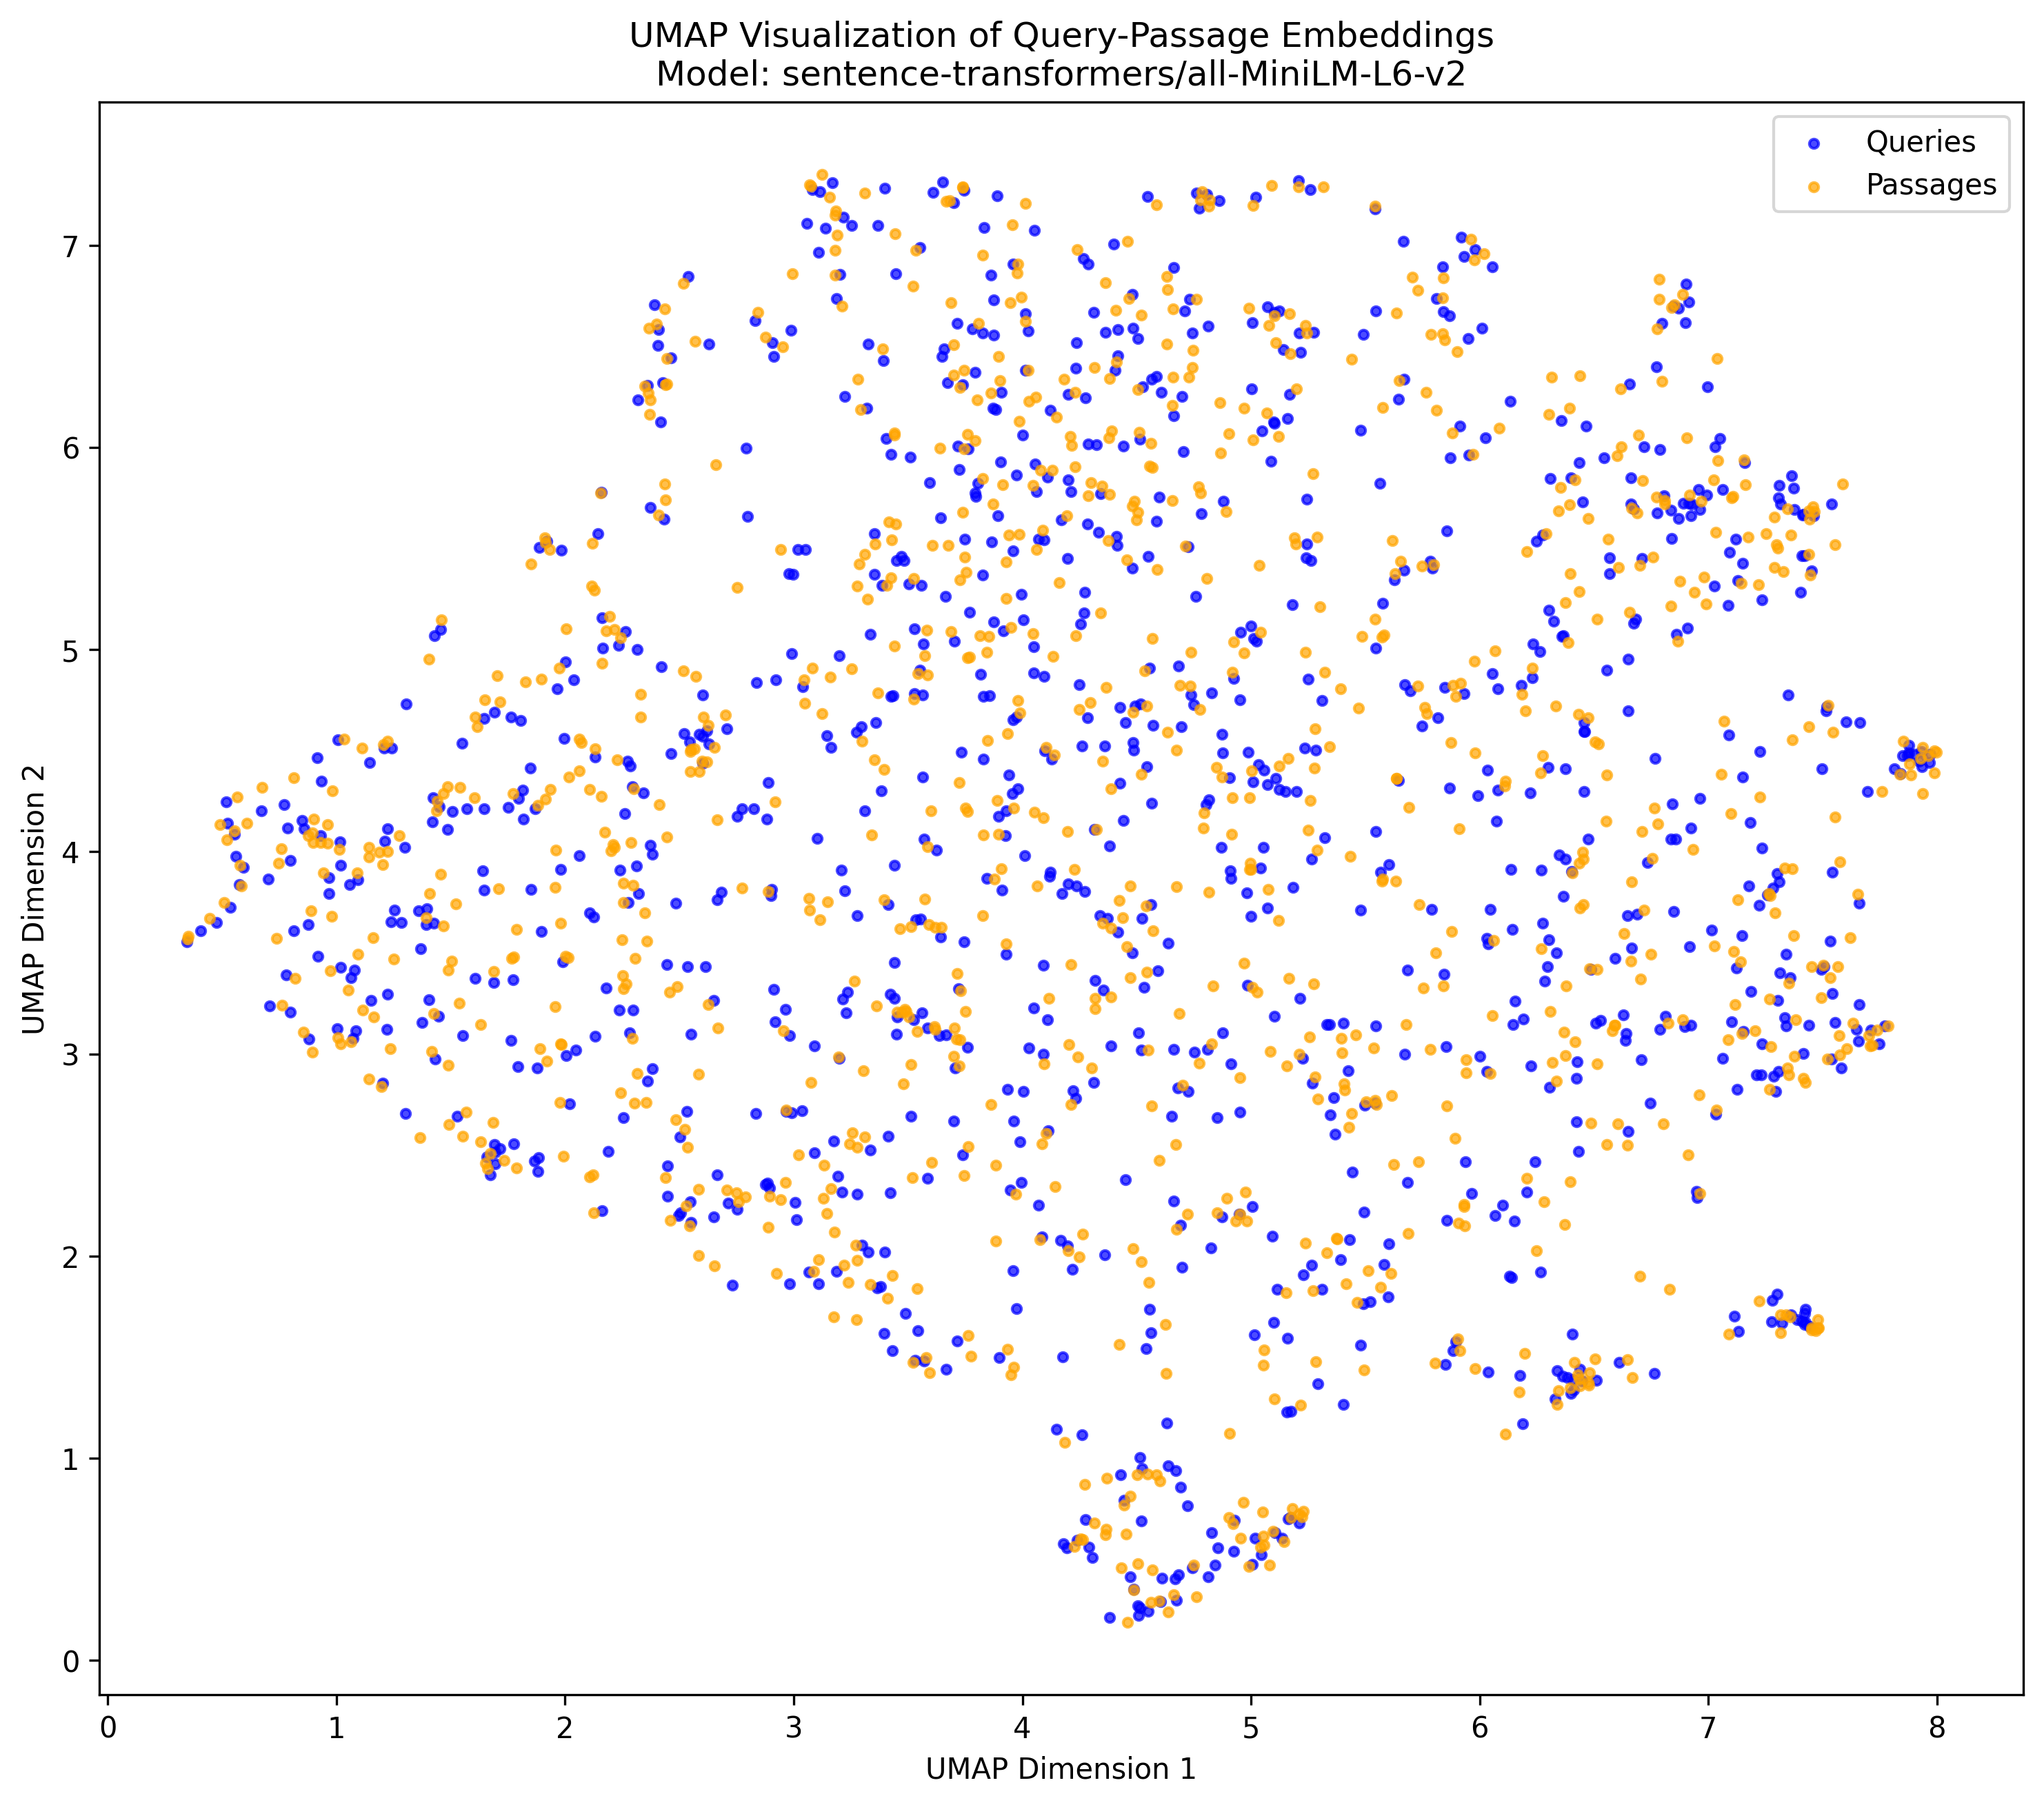
\includegraphics[width=\textwidth, height=0.75\textwidth, keepaspectratio]{umap_visualization_sentence_transformers_all_MiniLM_L6_v2.png}
\caption{Base SBERT: Well-defined semantic clustering with natural boundaries and balanced distribution}
\label{fig:umap_base_thesis}
\end{subfigure}
\hfill
\begin{subfigure}{0.48\textwidth}
\centering
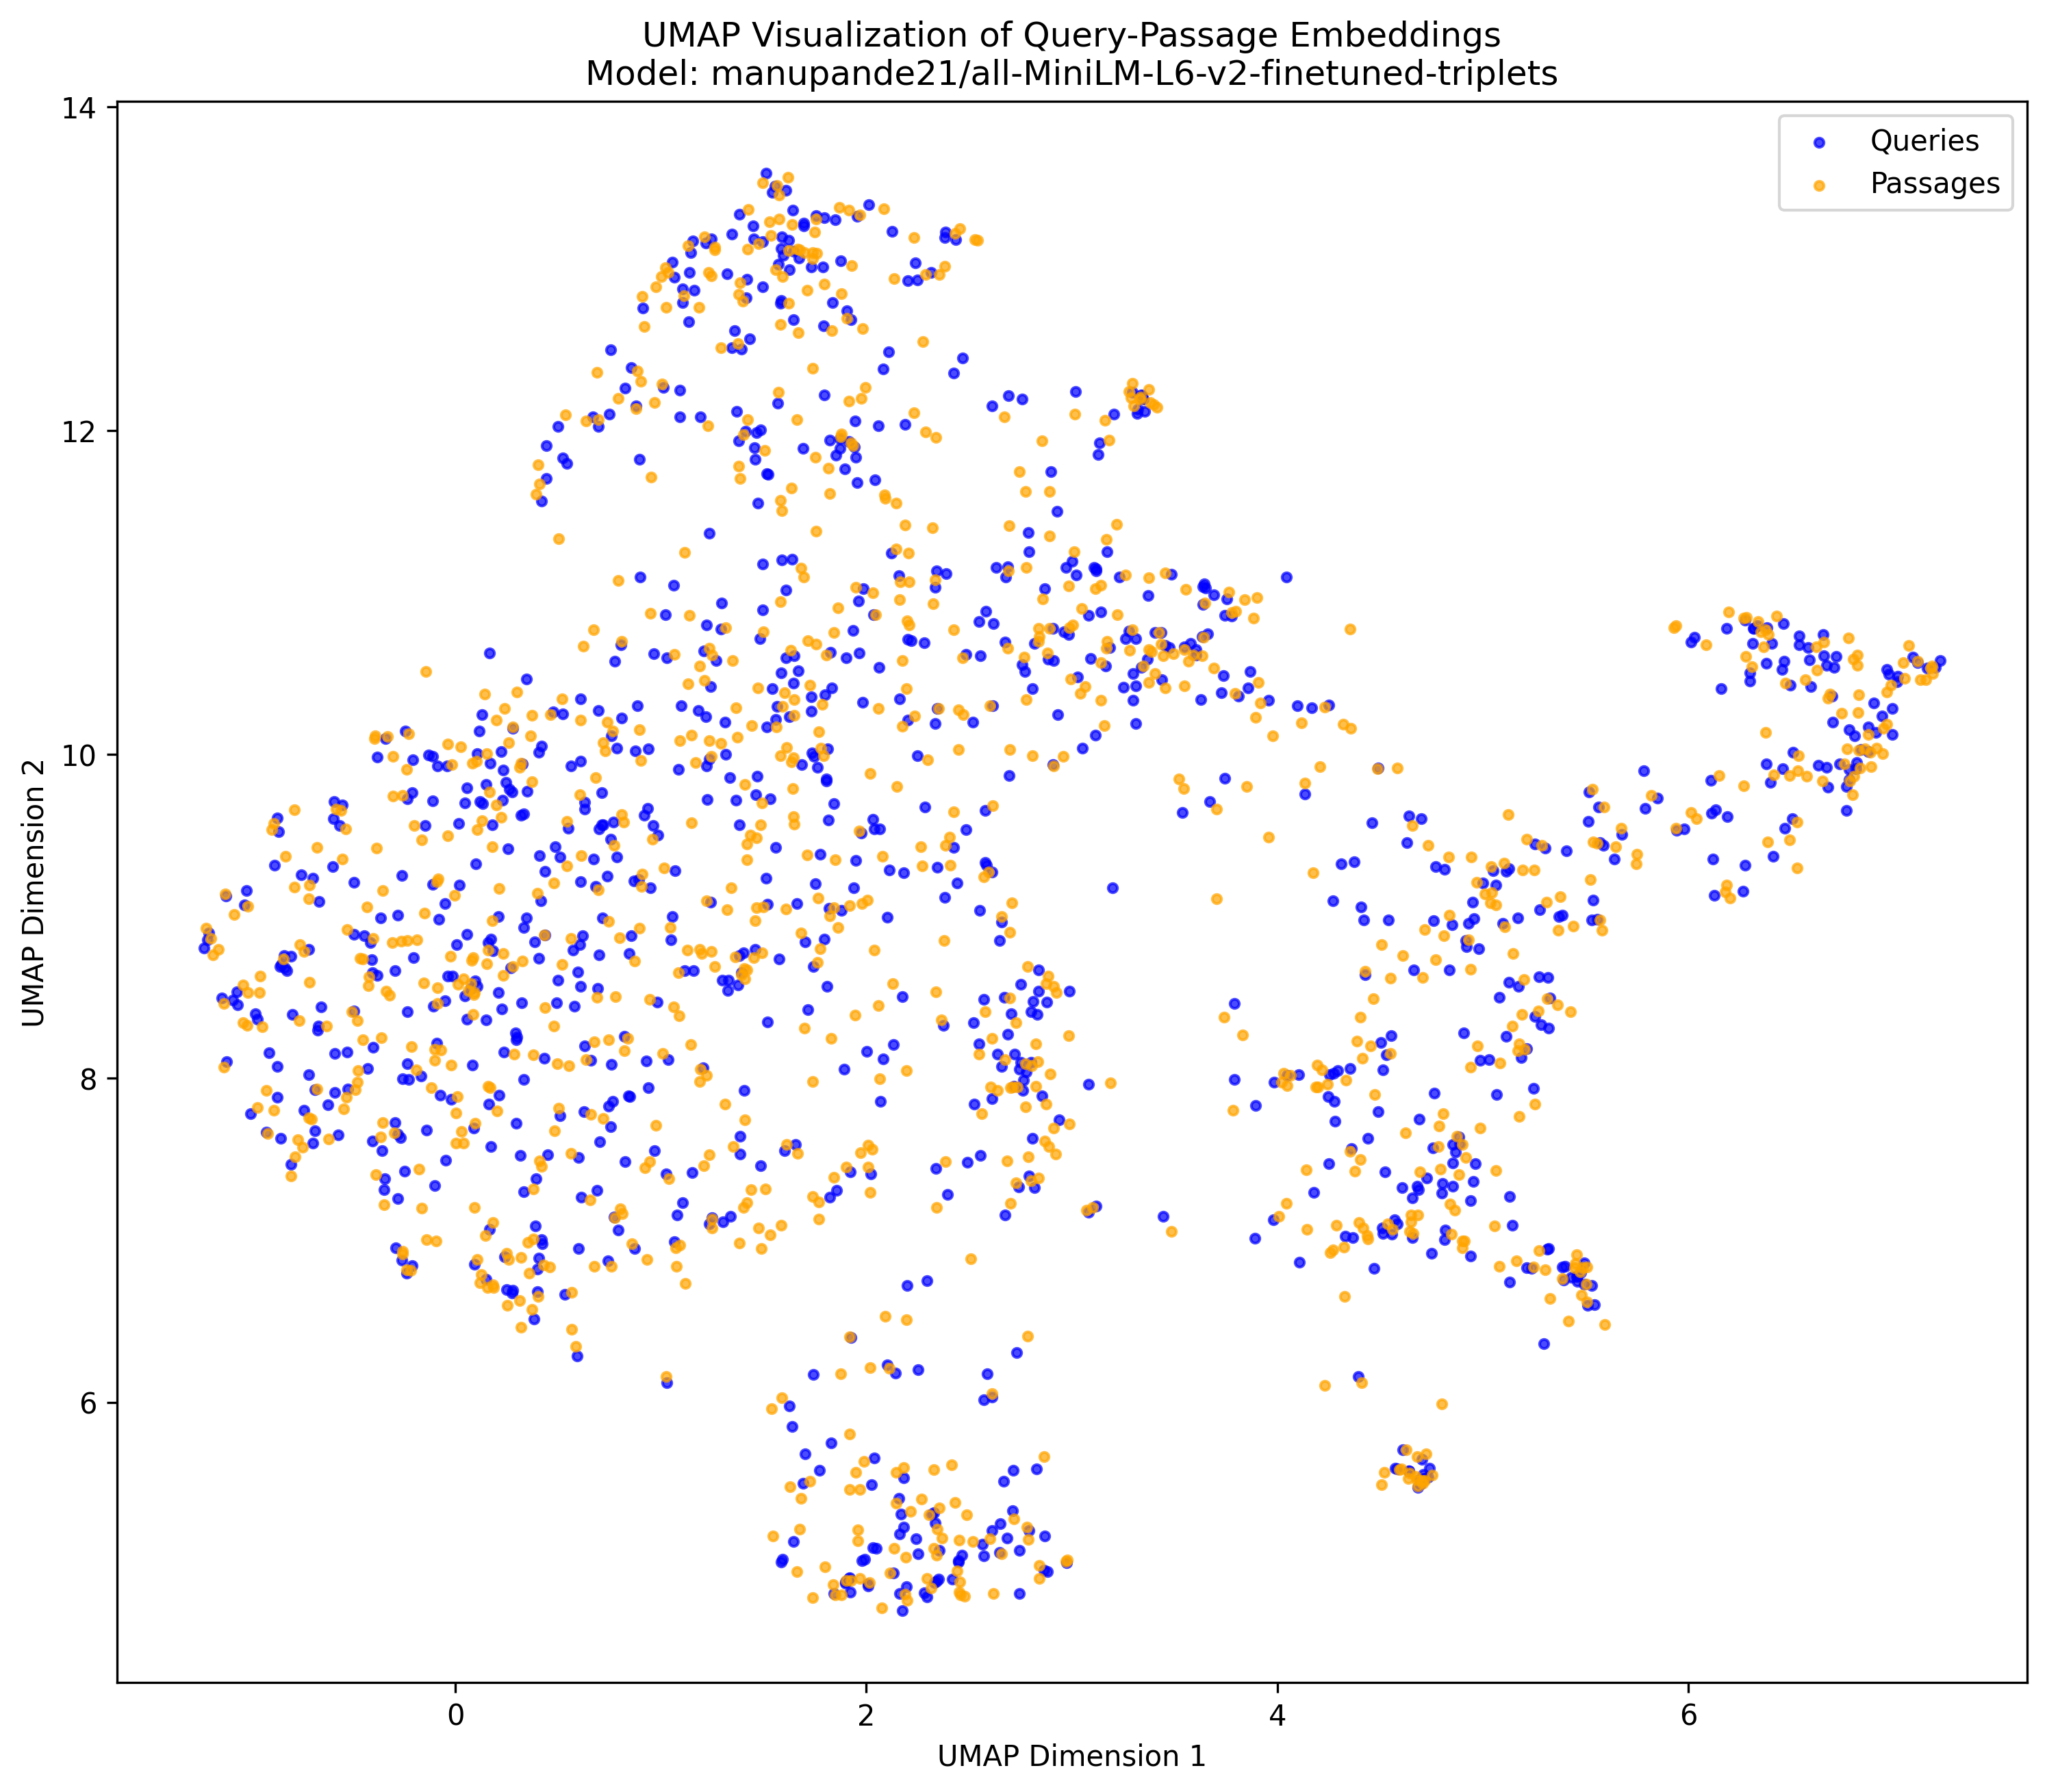
\includegraphics[width=\textwidth, height=0.75\textwidth, keepaspectratio]{umap_visualization_manupande21_all_MiniLM_L6_v2_finetuned_triplets.png}
\caption{Full FT (Random): Distinct island formations with preserved but altered clustering structure}
\label{fig:umap_full_random_thesis}
\end{subfigure}

\vspace{0.8cm}

% Second row: Full FT Hard and LoRA Random
\begin{subfigure}{0.48\textwidth}
\centering
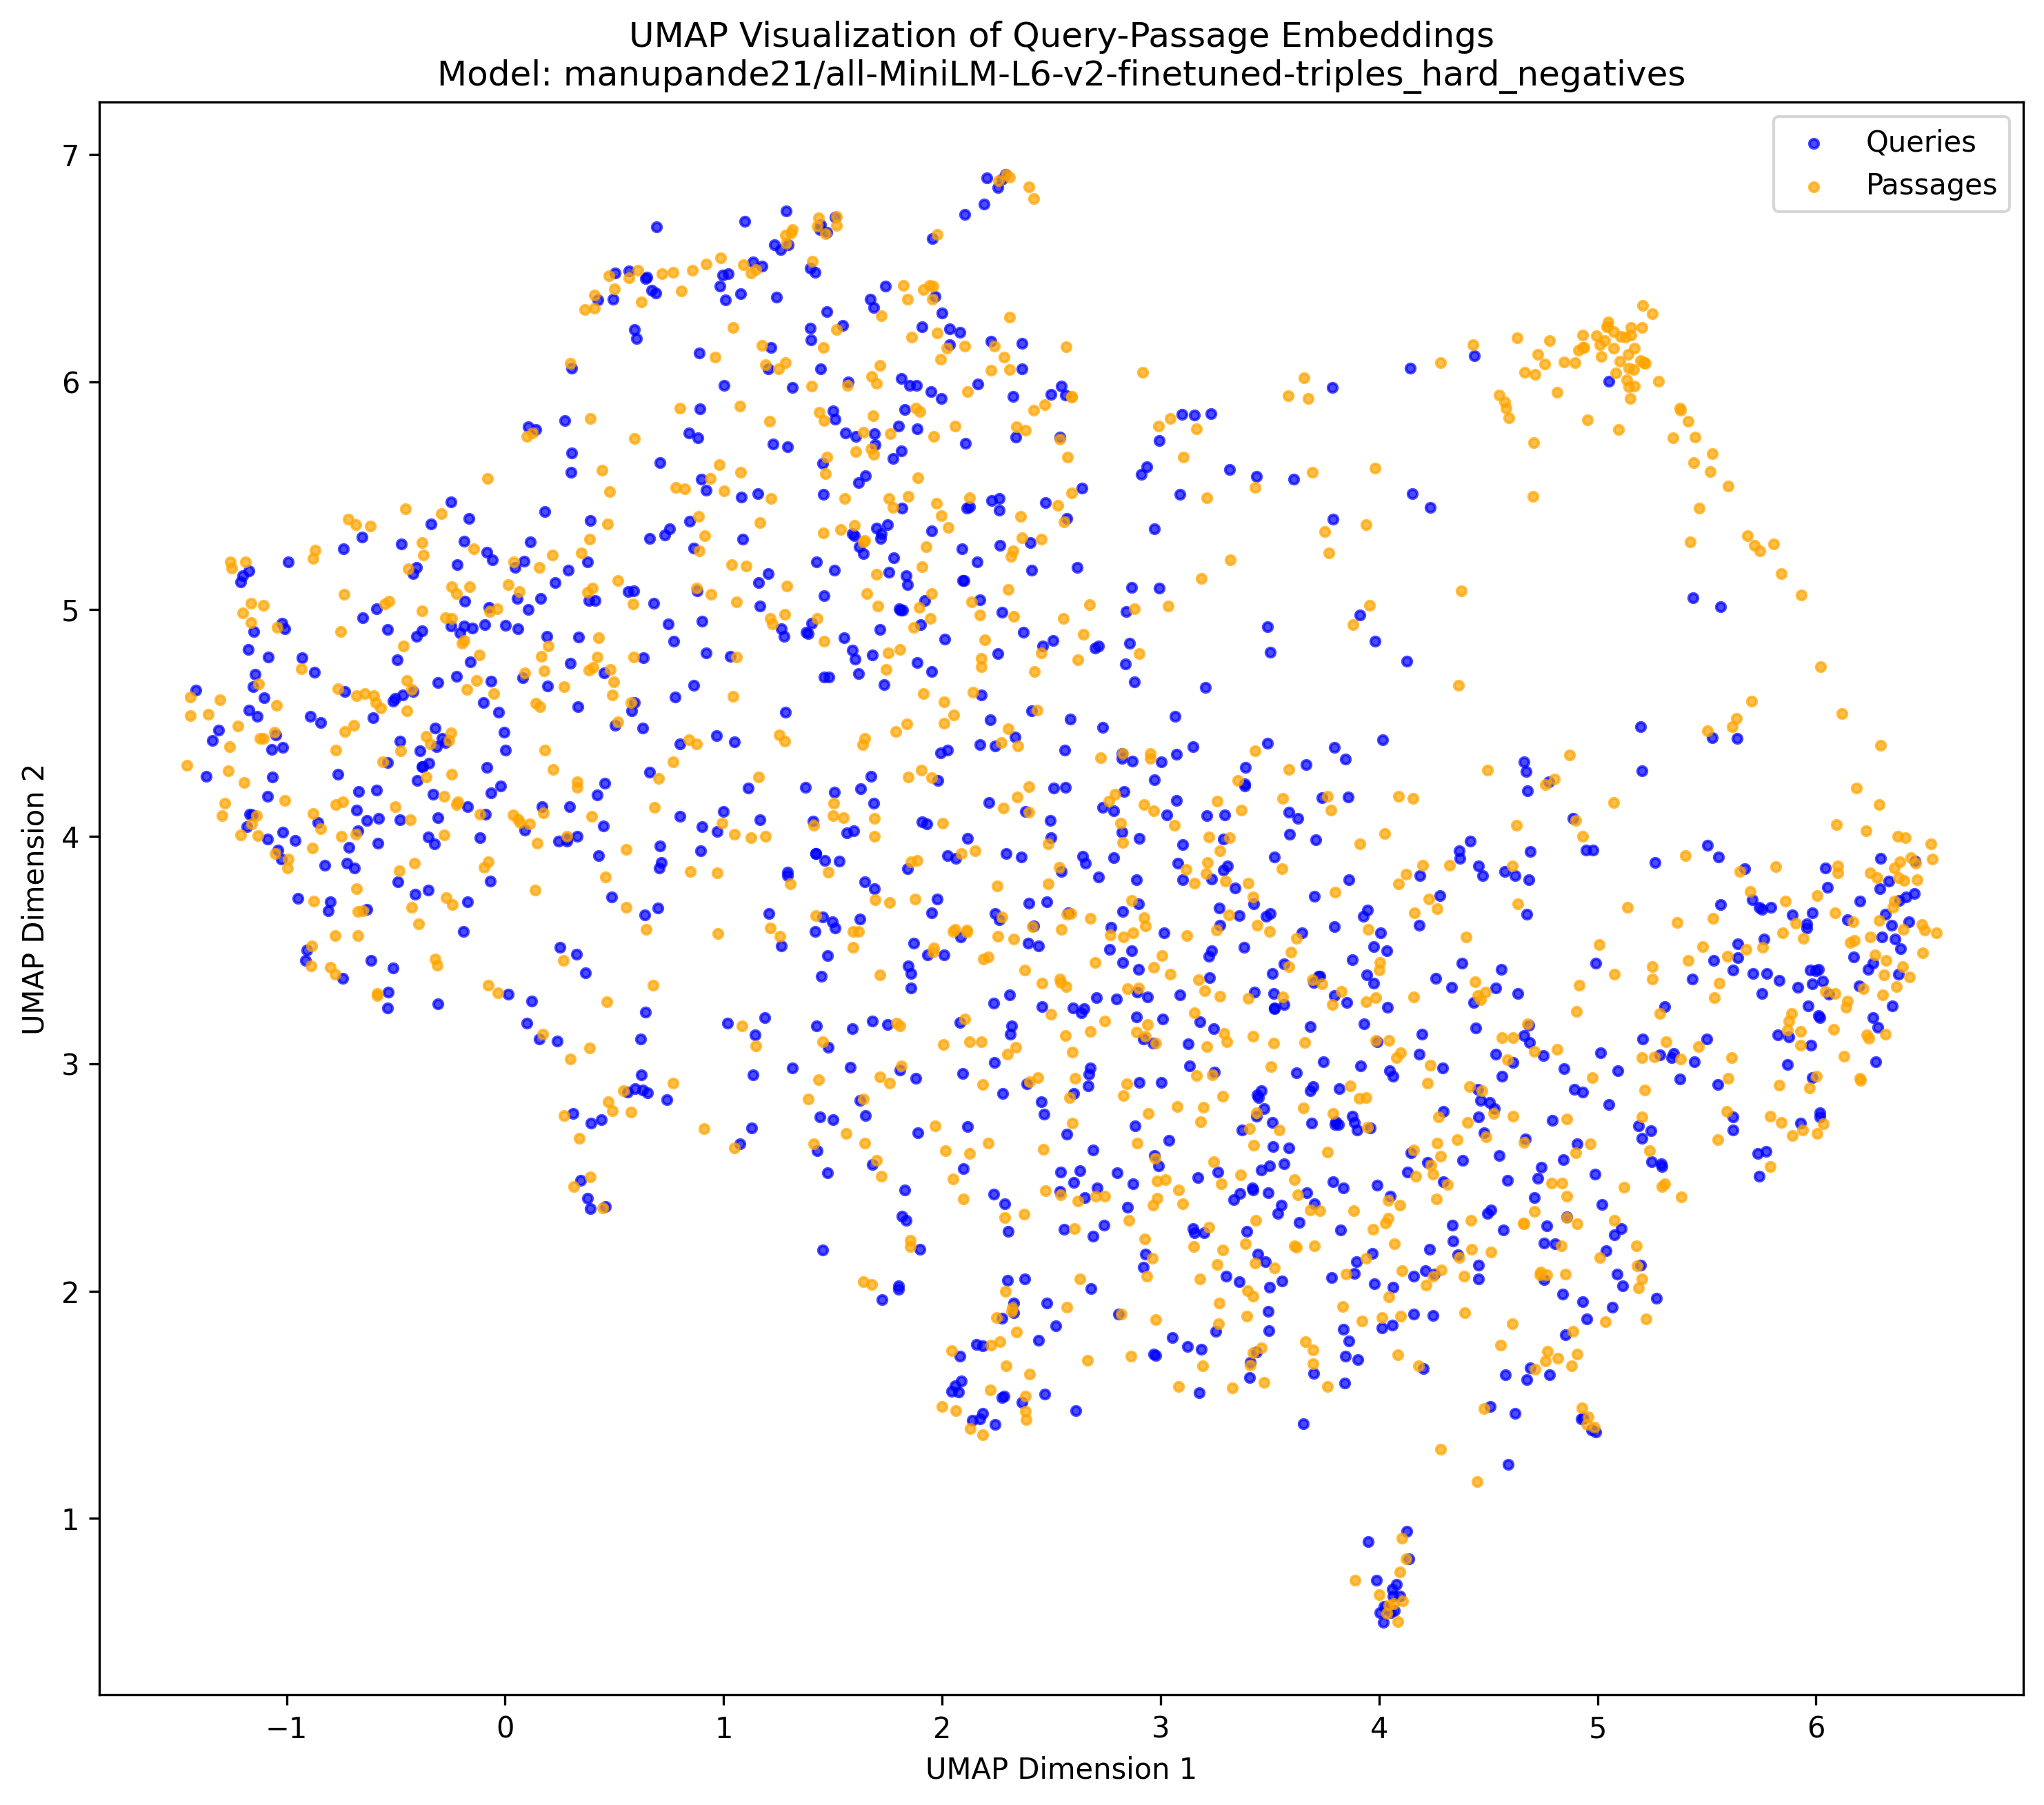
\includegraphics[width=\textwidth, height=0.75\textwidth, keepaspectratio]{umap_visualization_manupande21_all_MiniLM_L6_v2_finetuned_triples_hard_negatives.png}
\caption{Full FT (Hard): Increased uniformity showing moderate embedding space flattening}
\label{fig:umap_full_hard_thesis}
\end{subfigure}
\hfill
\begin{subfigure}{0.48\textwidth}
\centering
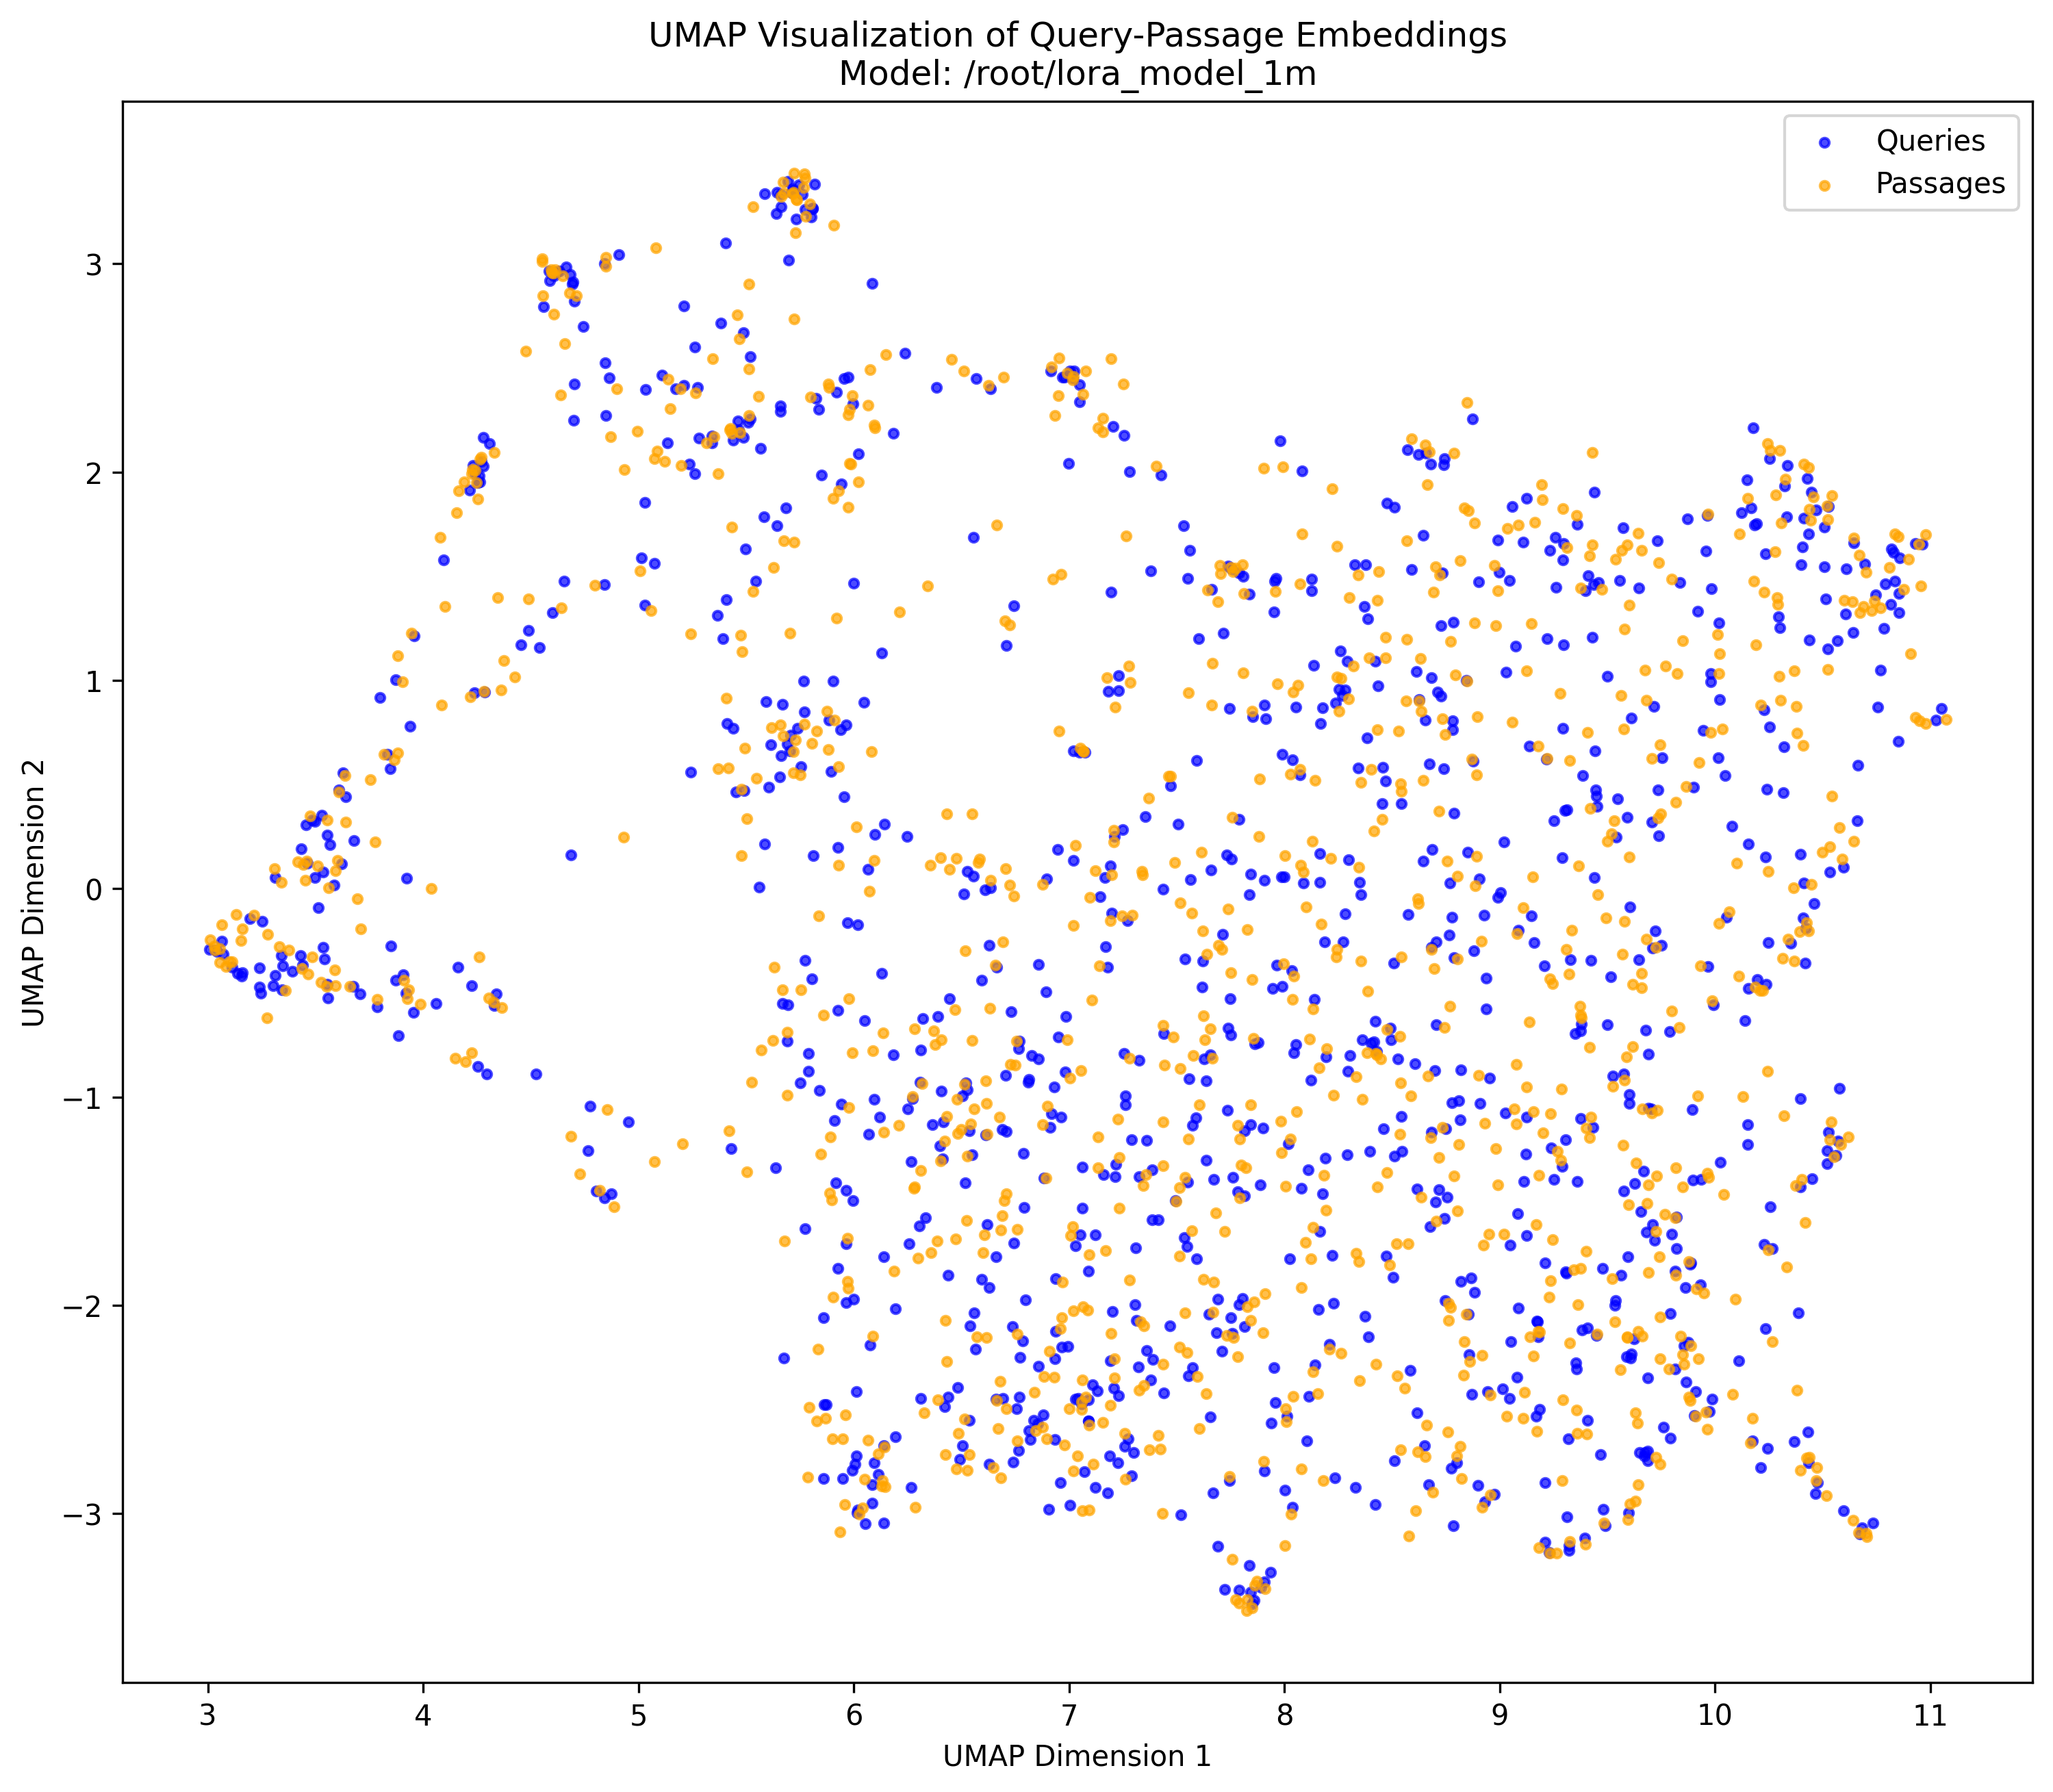
\includegraphics[width=\textwidth, height=0.75\textwidth, keepaspectratio]{umap_visualization__root_lora_model_1m.png}
\caption{LoRA FT (Random): Reduced semantic differentiation with compressed clustering}
\label{fig:umap_lora_random_thesis}
\end{subfigure}

\vspace{0.8cm}

% Third row: LoRA Hard (centered)
\begin{subfigure}{0.48\textwidth}
\centering
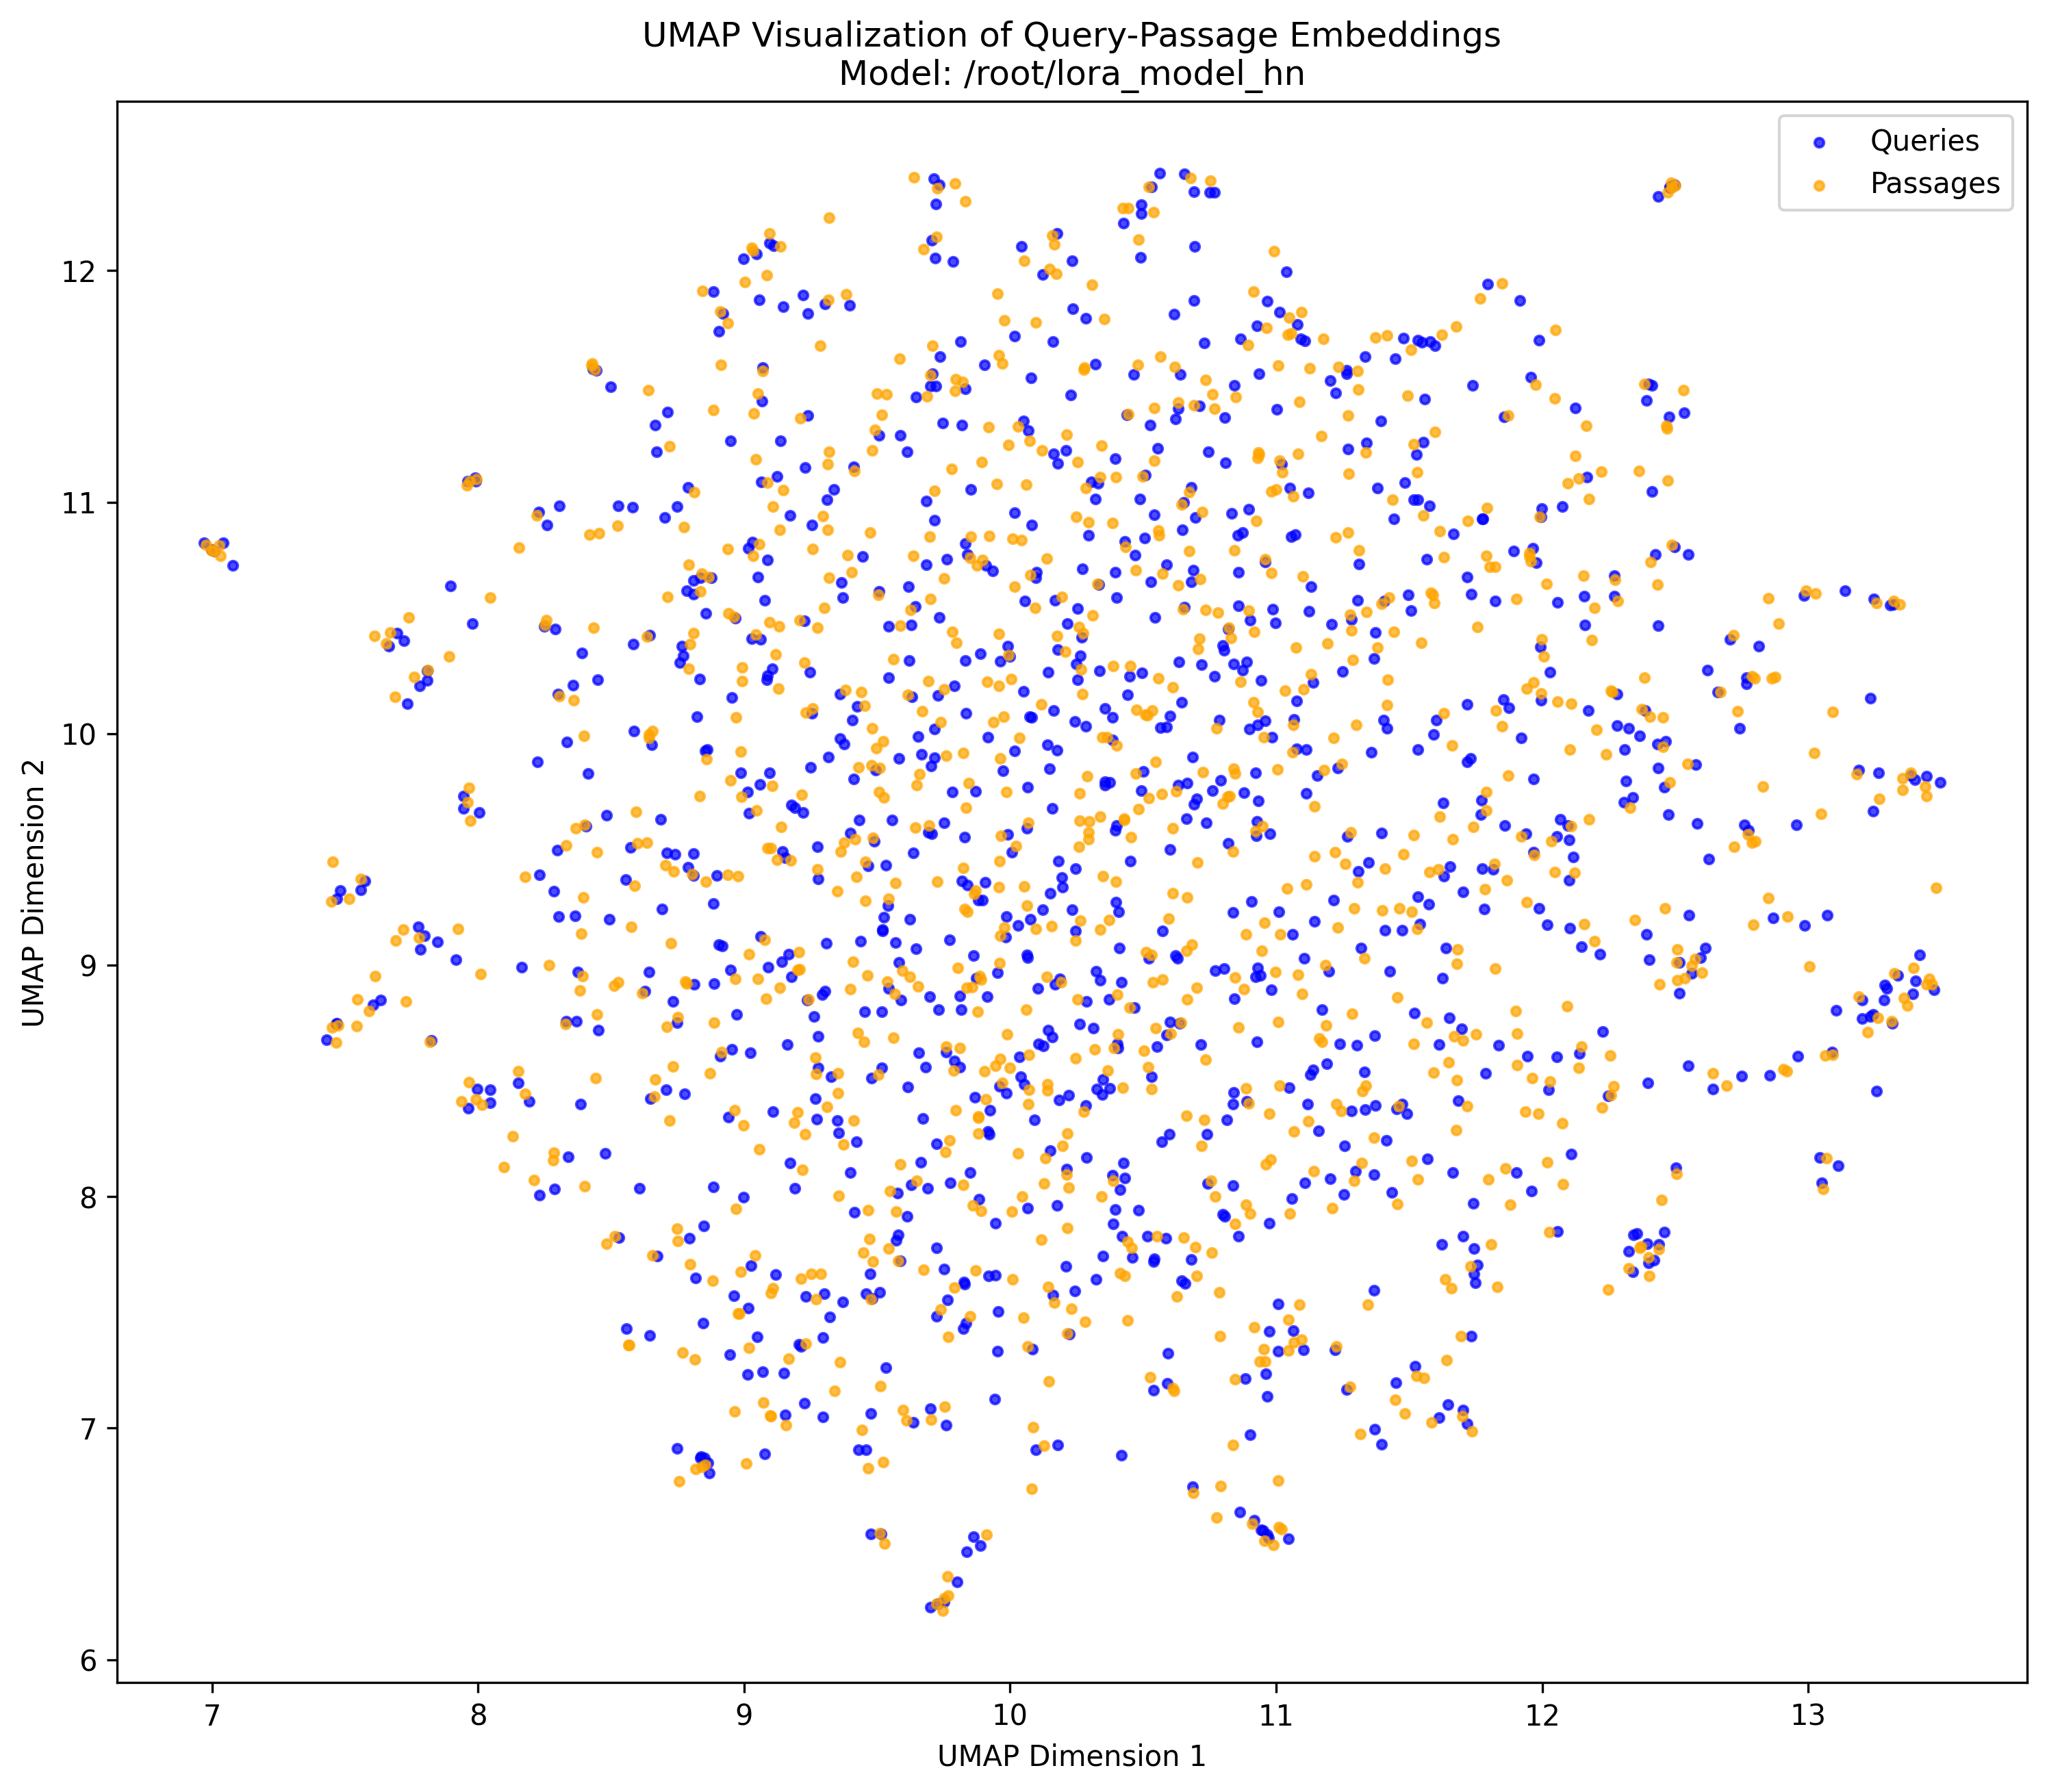
\includegraphics[width=\textwidth, height=0.75\textwidth, keepaspectratio]{umap_visualization__root_lora_model_hn.png}
\caption{LoRA FT (Hard): Maximum uniformity demonstrating catastrophic embedding space collapse}
\label{fig:umap_lora_hard_thesis}
\end{subfigure}

\caption{UMAP visualization of embedding spaces. Blue points represent query embeddings and orange points represent positive passage embeddings from 1,000 randomly sampled query-passage pairs. The progression demonstrates increasing embedding space uniformity.}
\label{fig:umap_all_thesis}
\end{figure*}

The visualization reveals a clear degradation progression: from well-structured semantic organization in the base model to complete uniformity in LoRA Hard, demonstrating how fine-tuning progressively degrades embedding space structure.

\section{Training Dynamics Analysis}

Figure~\ref{fig:training_curves_thesis} shows training loss trajectories, with LoRA Hard exhibiting training instability and poor convergence, while Full FT Random achieves smooth optimization.

\begin{figure*}[t]
\centering
\begin{subfigure}{0.48\textwidth}
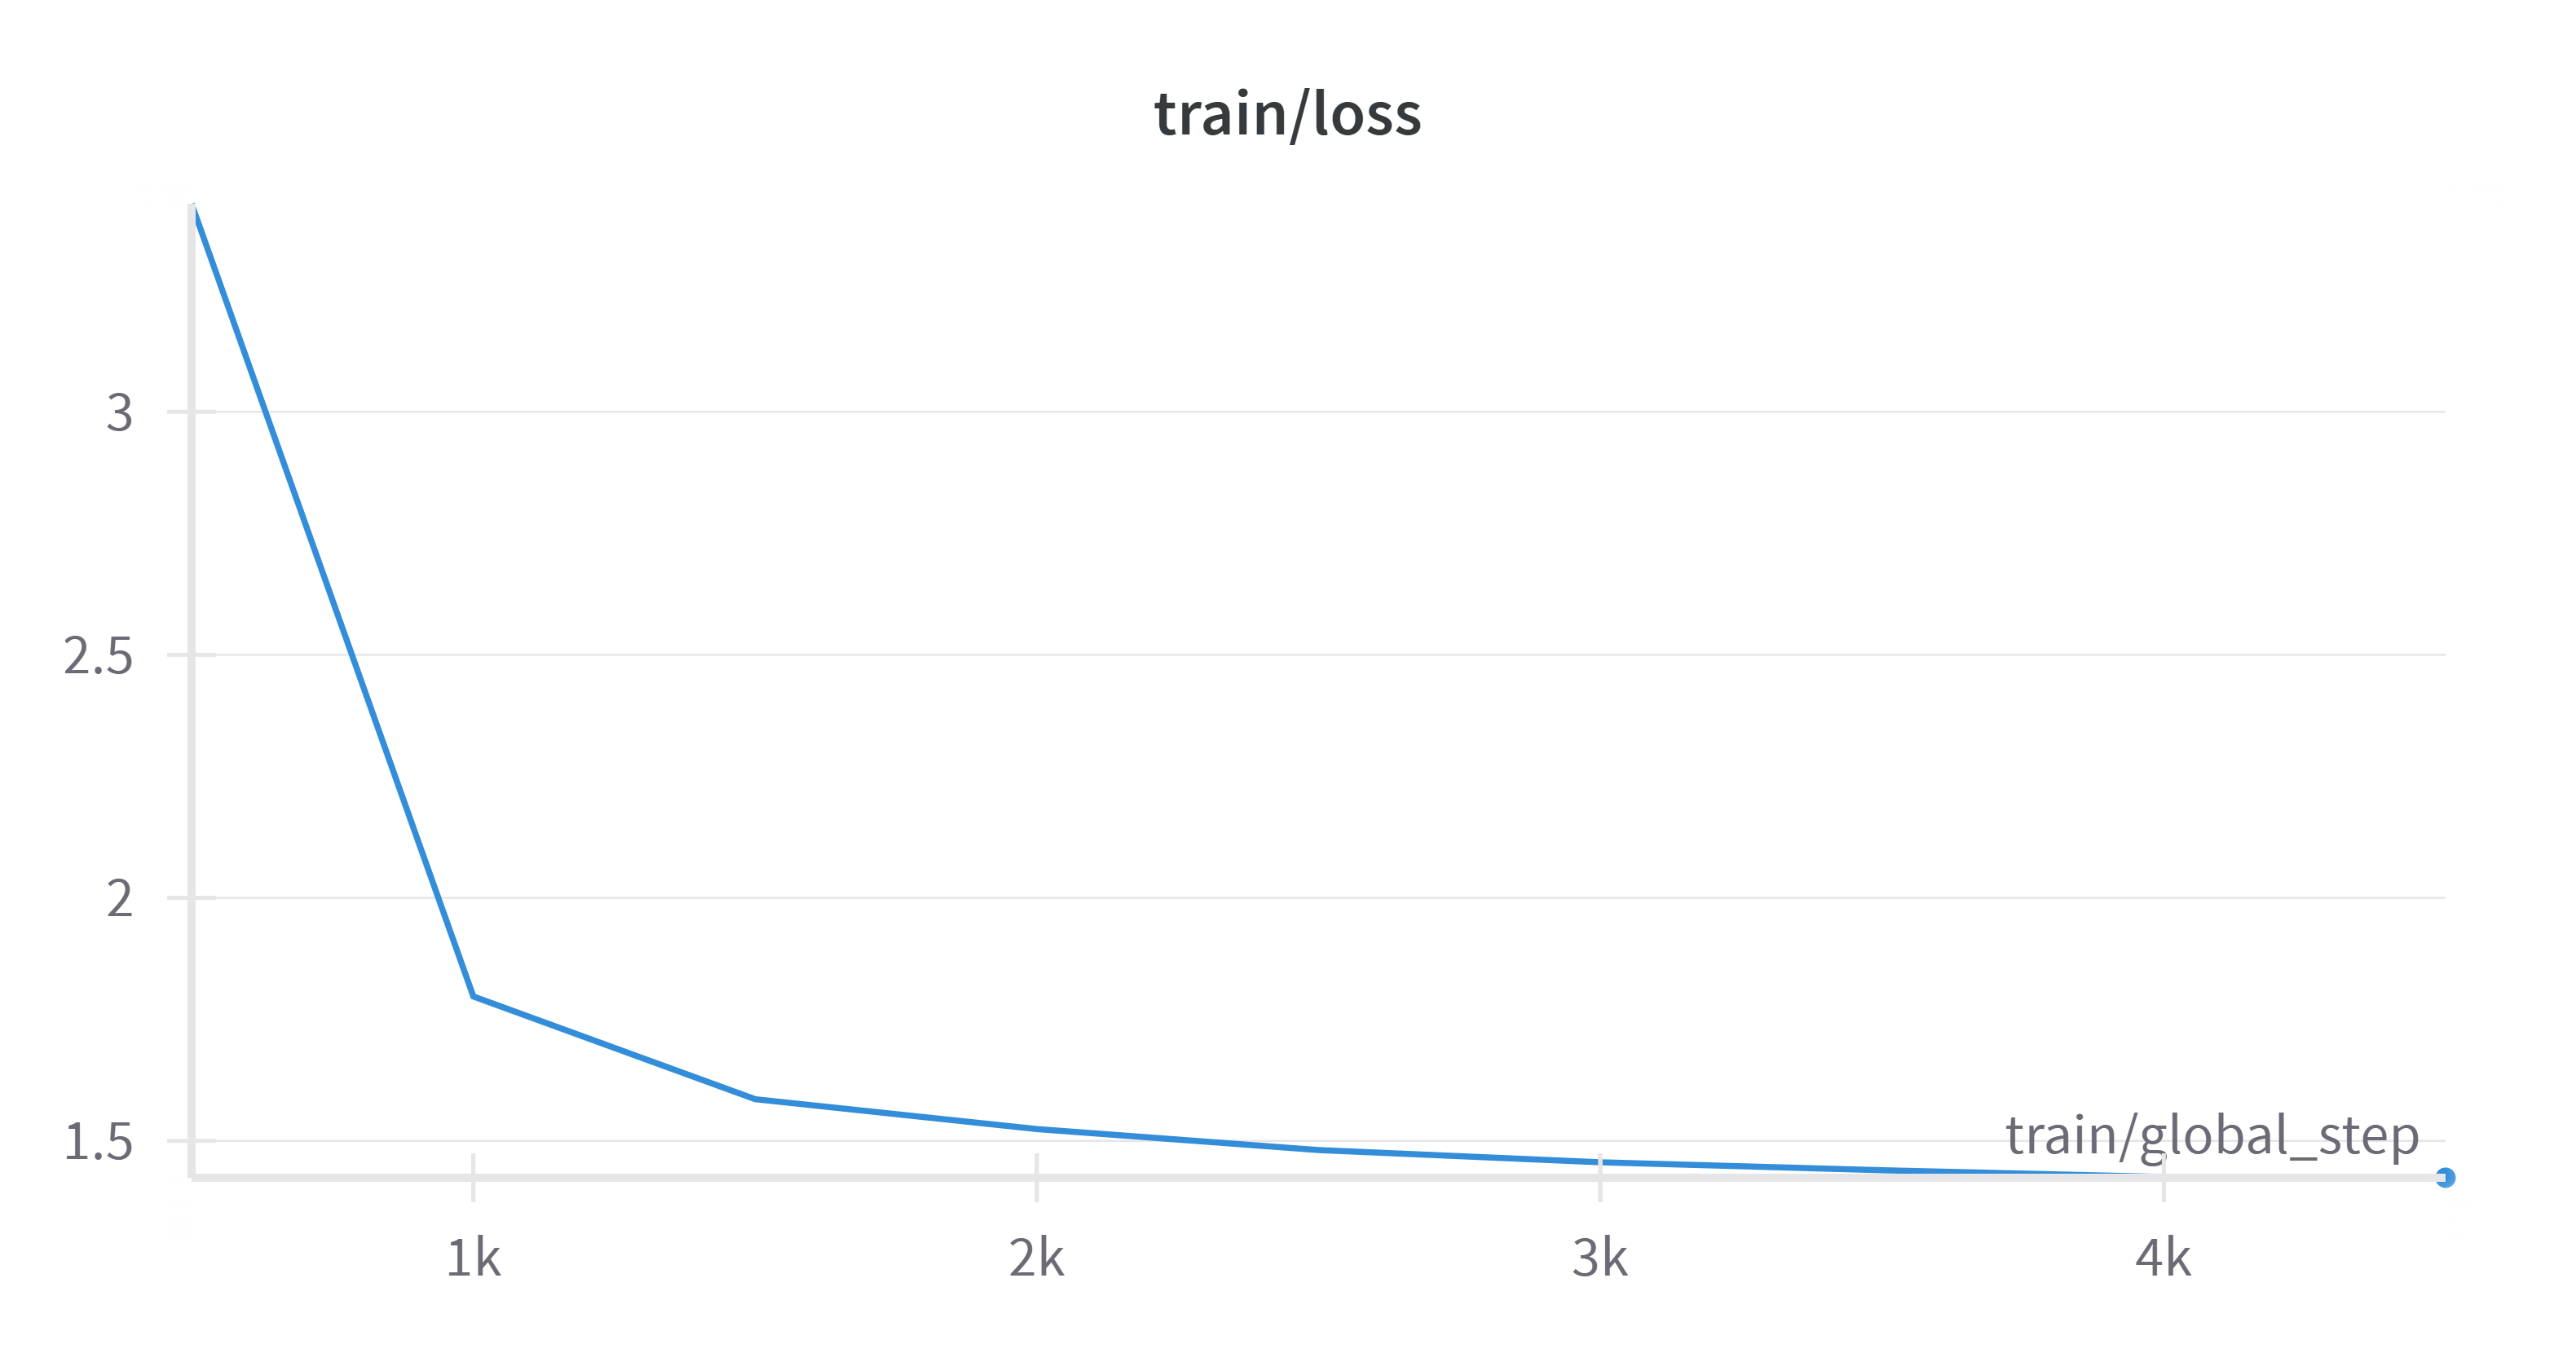
\includegraphics[width=\textwidth]{lora_finetuned_1million.png}
\caption{LoRA FT (Random): Steady convergence but higher final loss compared to full fine-tuning}
\end{subfigure}
\hfill
\begin{subfigure}{0.48\textwidth}
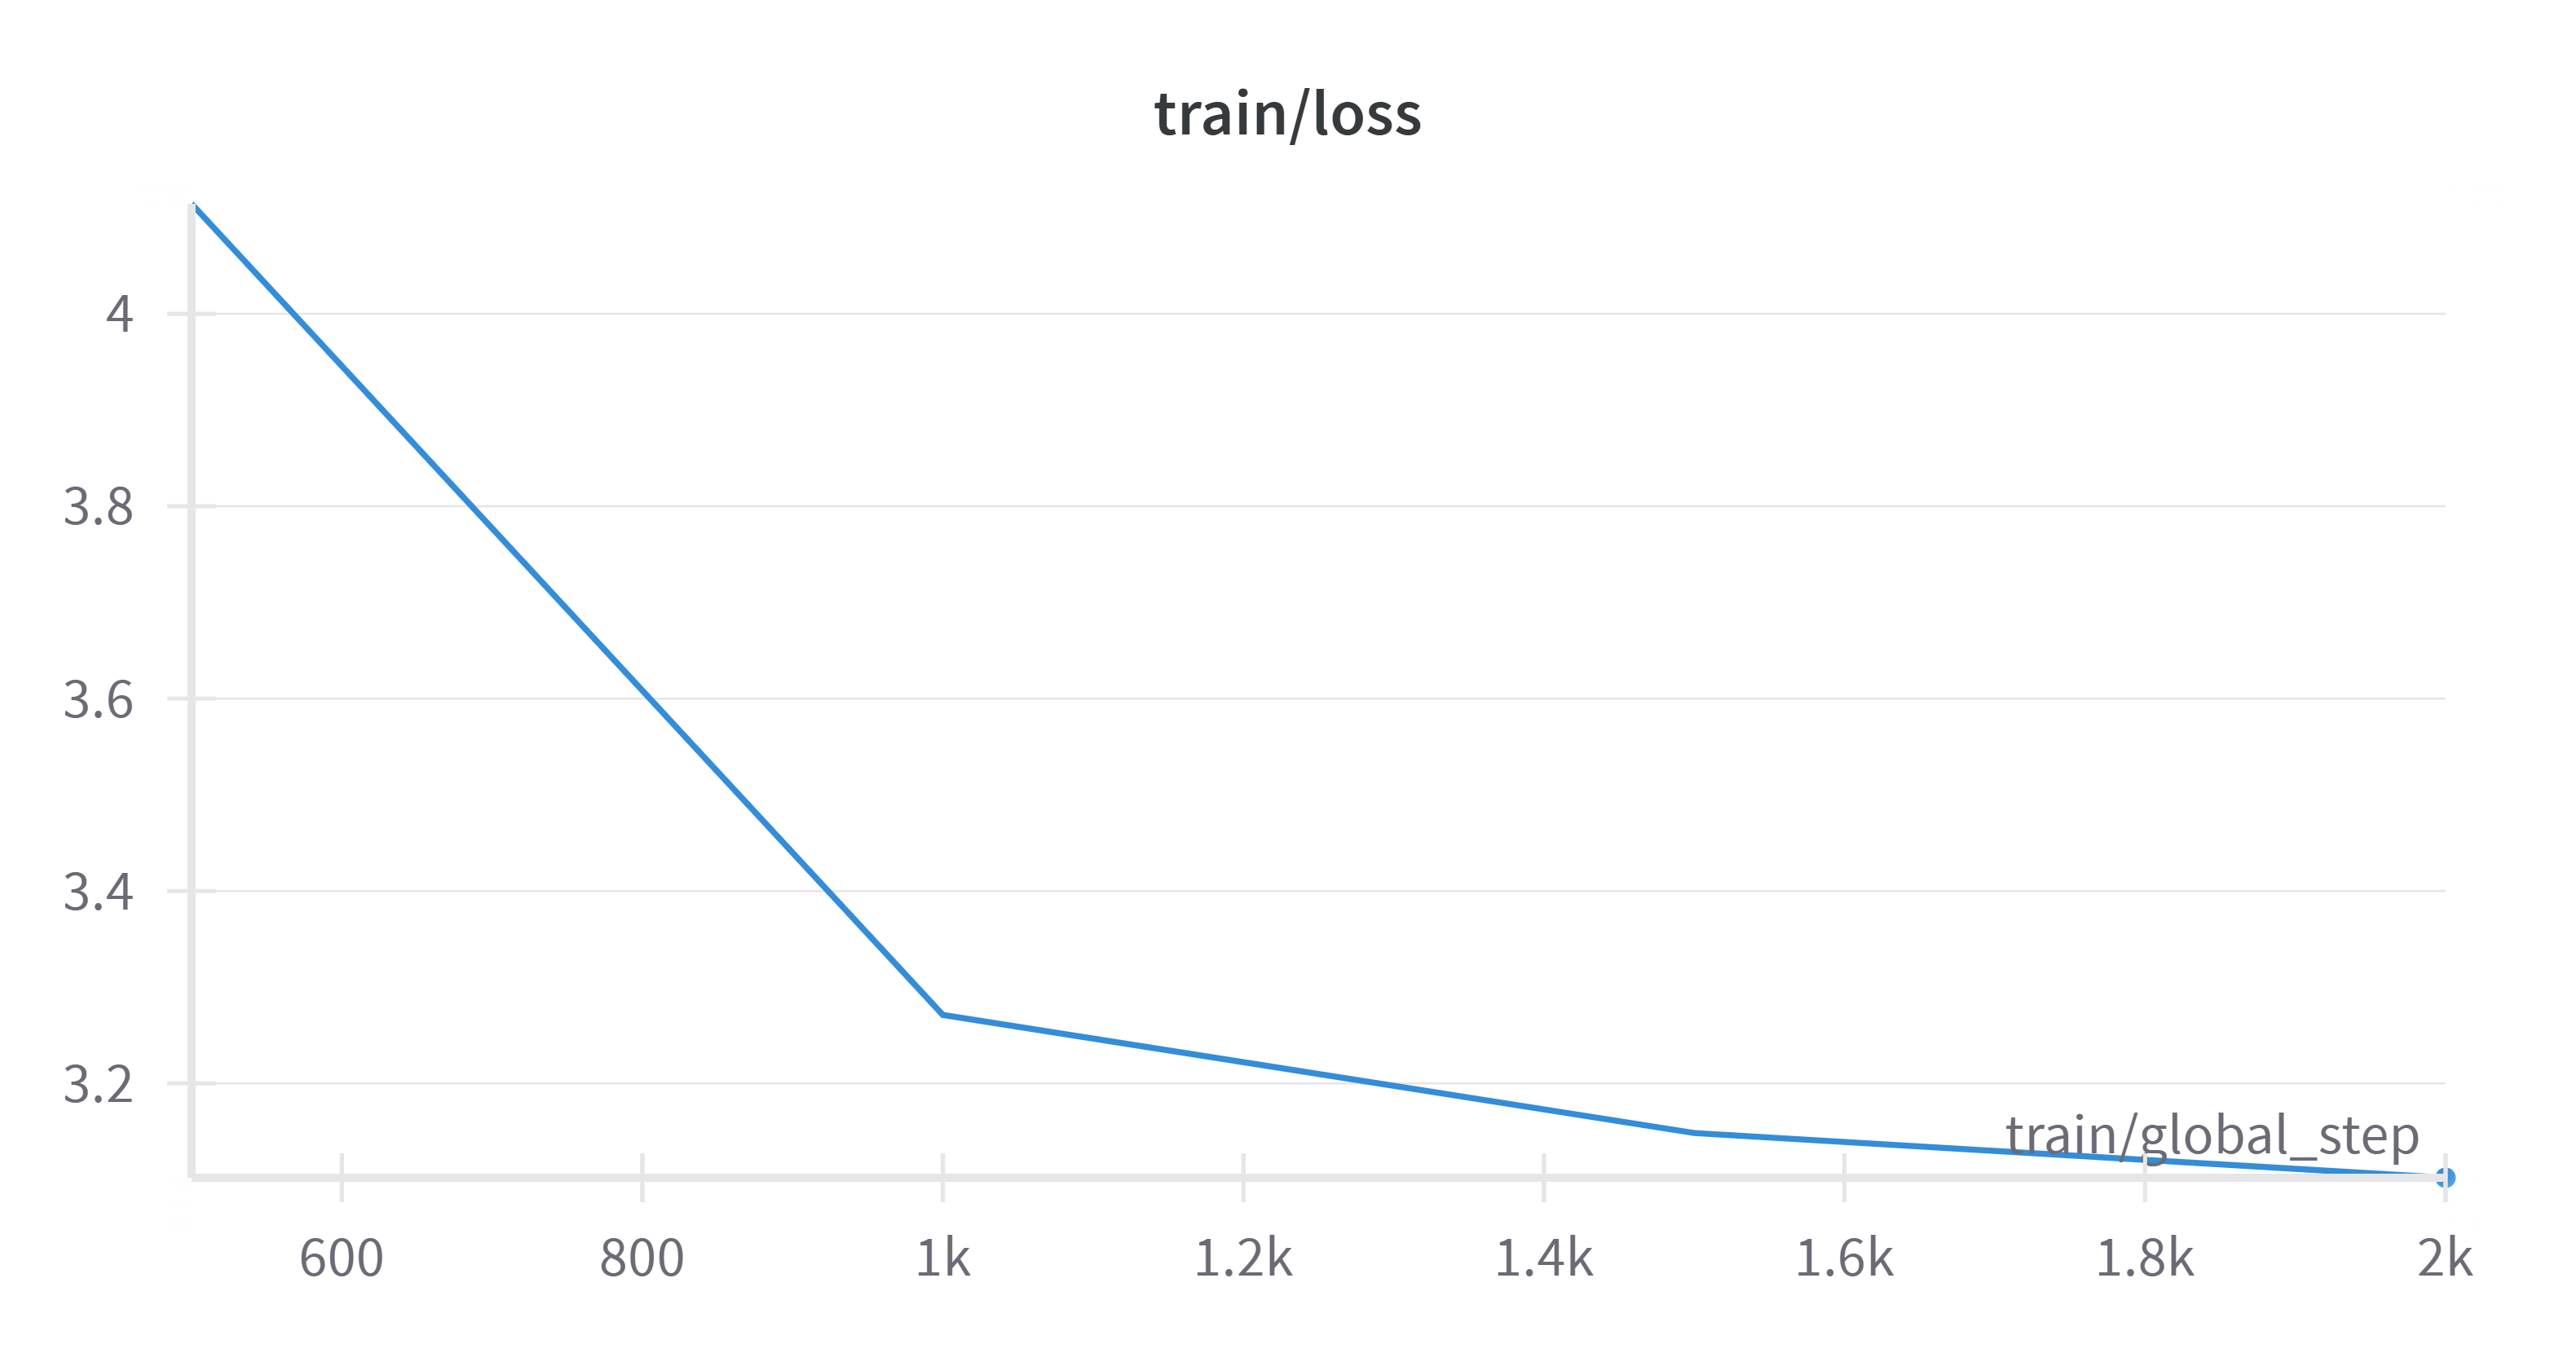
\includegraphics[width=\textwidth]{lora_finetuned_hard_negatives.png}
\caption{LoRA FT (Hard): Training instability and poor convergence leading to highest final loss}
\end{subfigure}

\begin{subfigure}{0.48\textwidth}
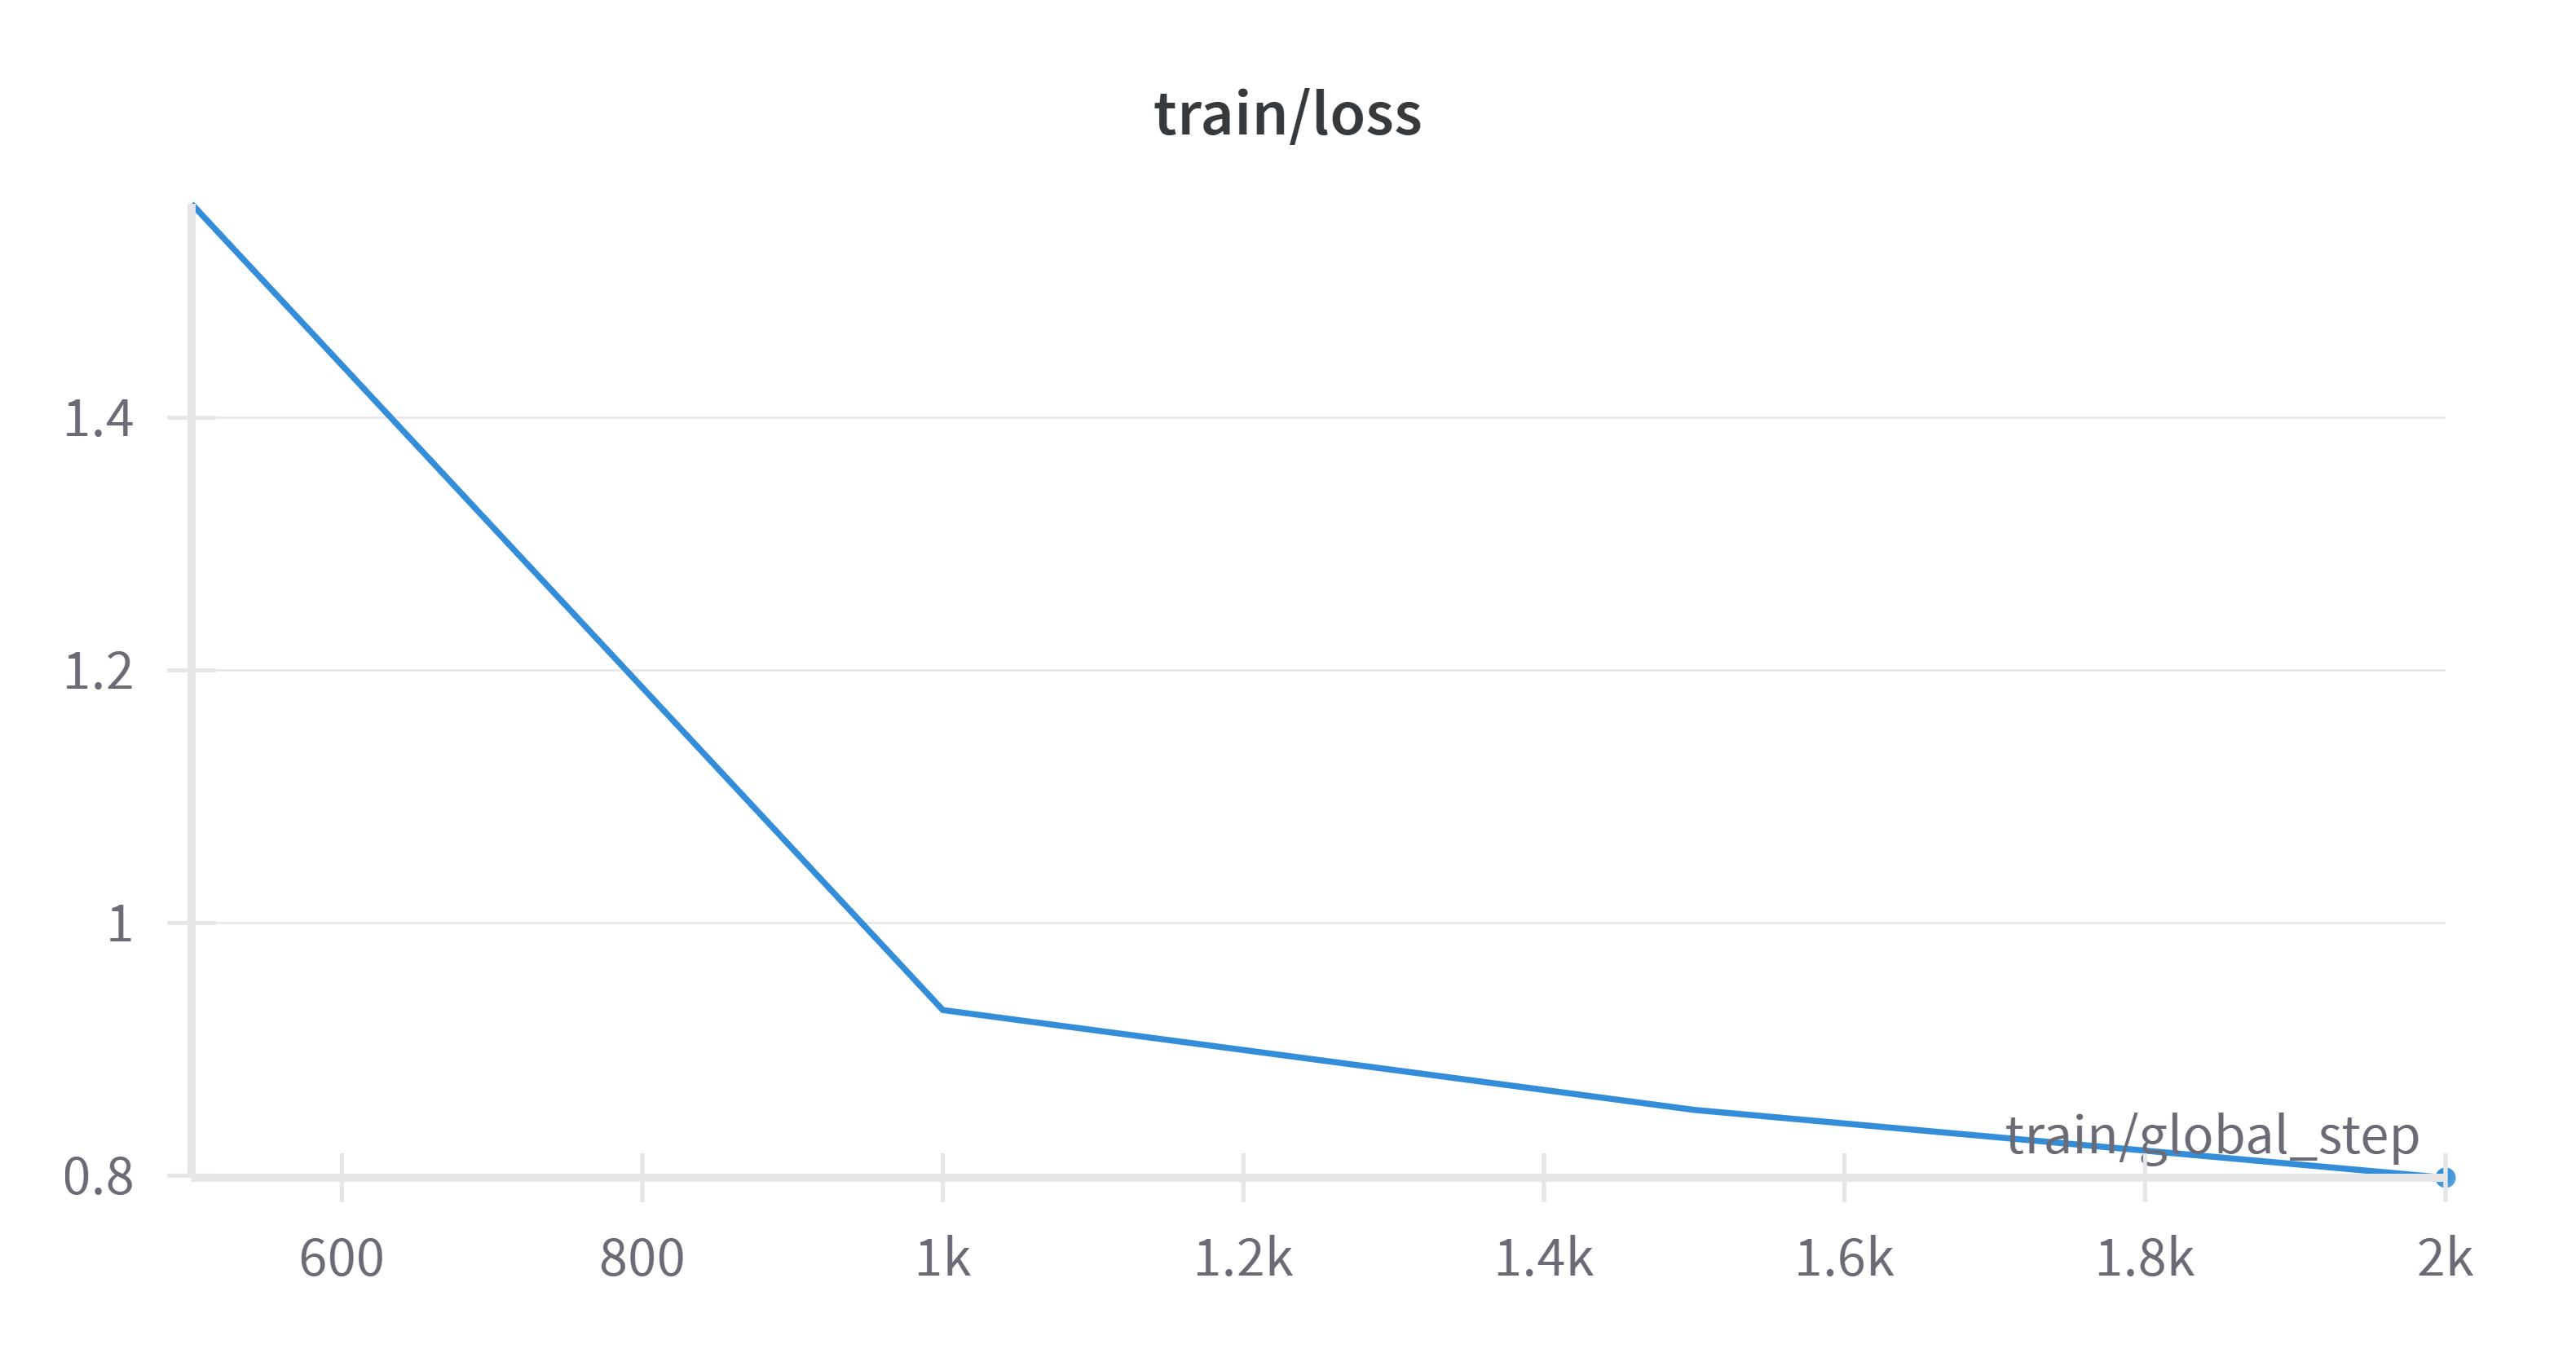
\includegraphics[width=\textwidth]{sbert_finetuned_1million.png}
\caption{Full FT (Random): Smooth optimization achieving lowest training loss across all variants}
\end{subfigure}
\hfill
\begin{subfigure}{0.48\textwidth}
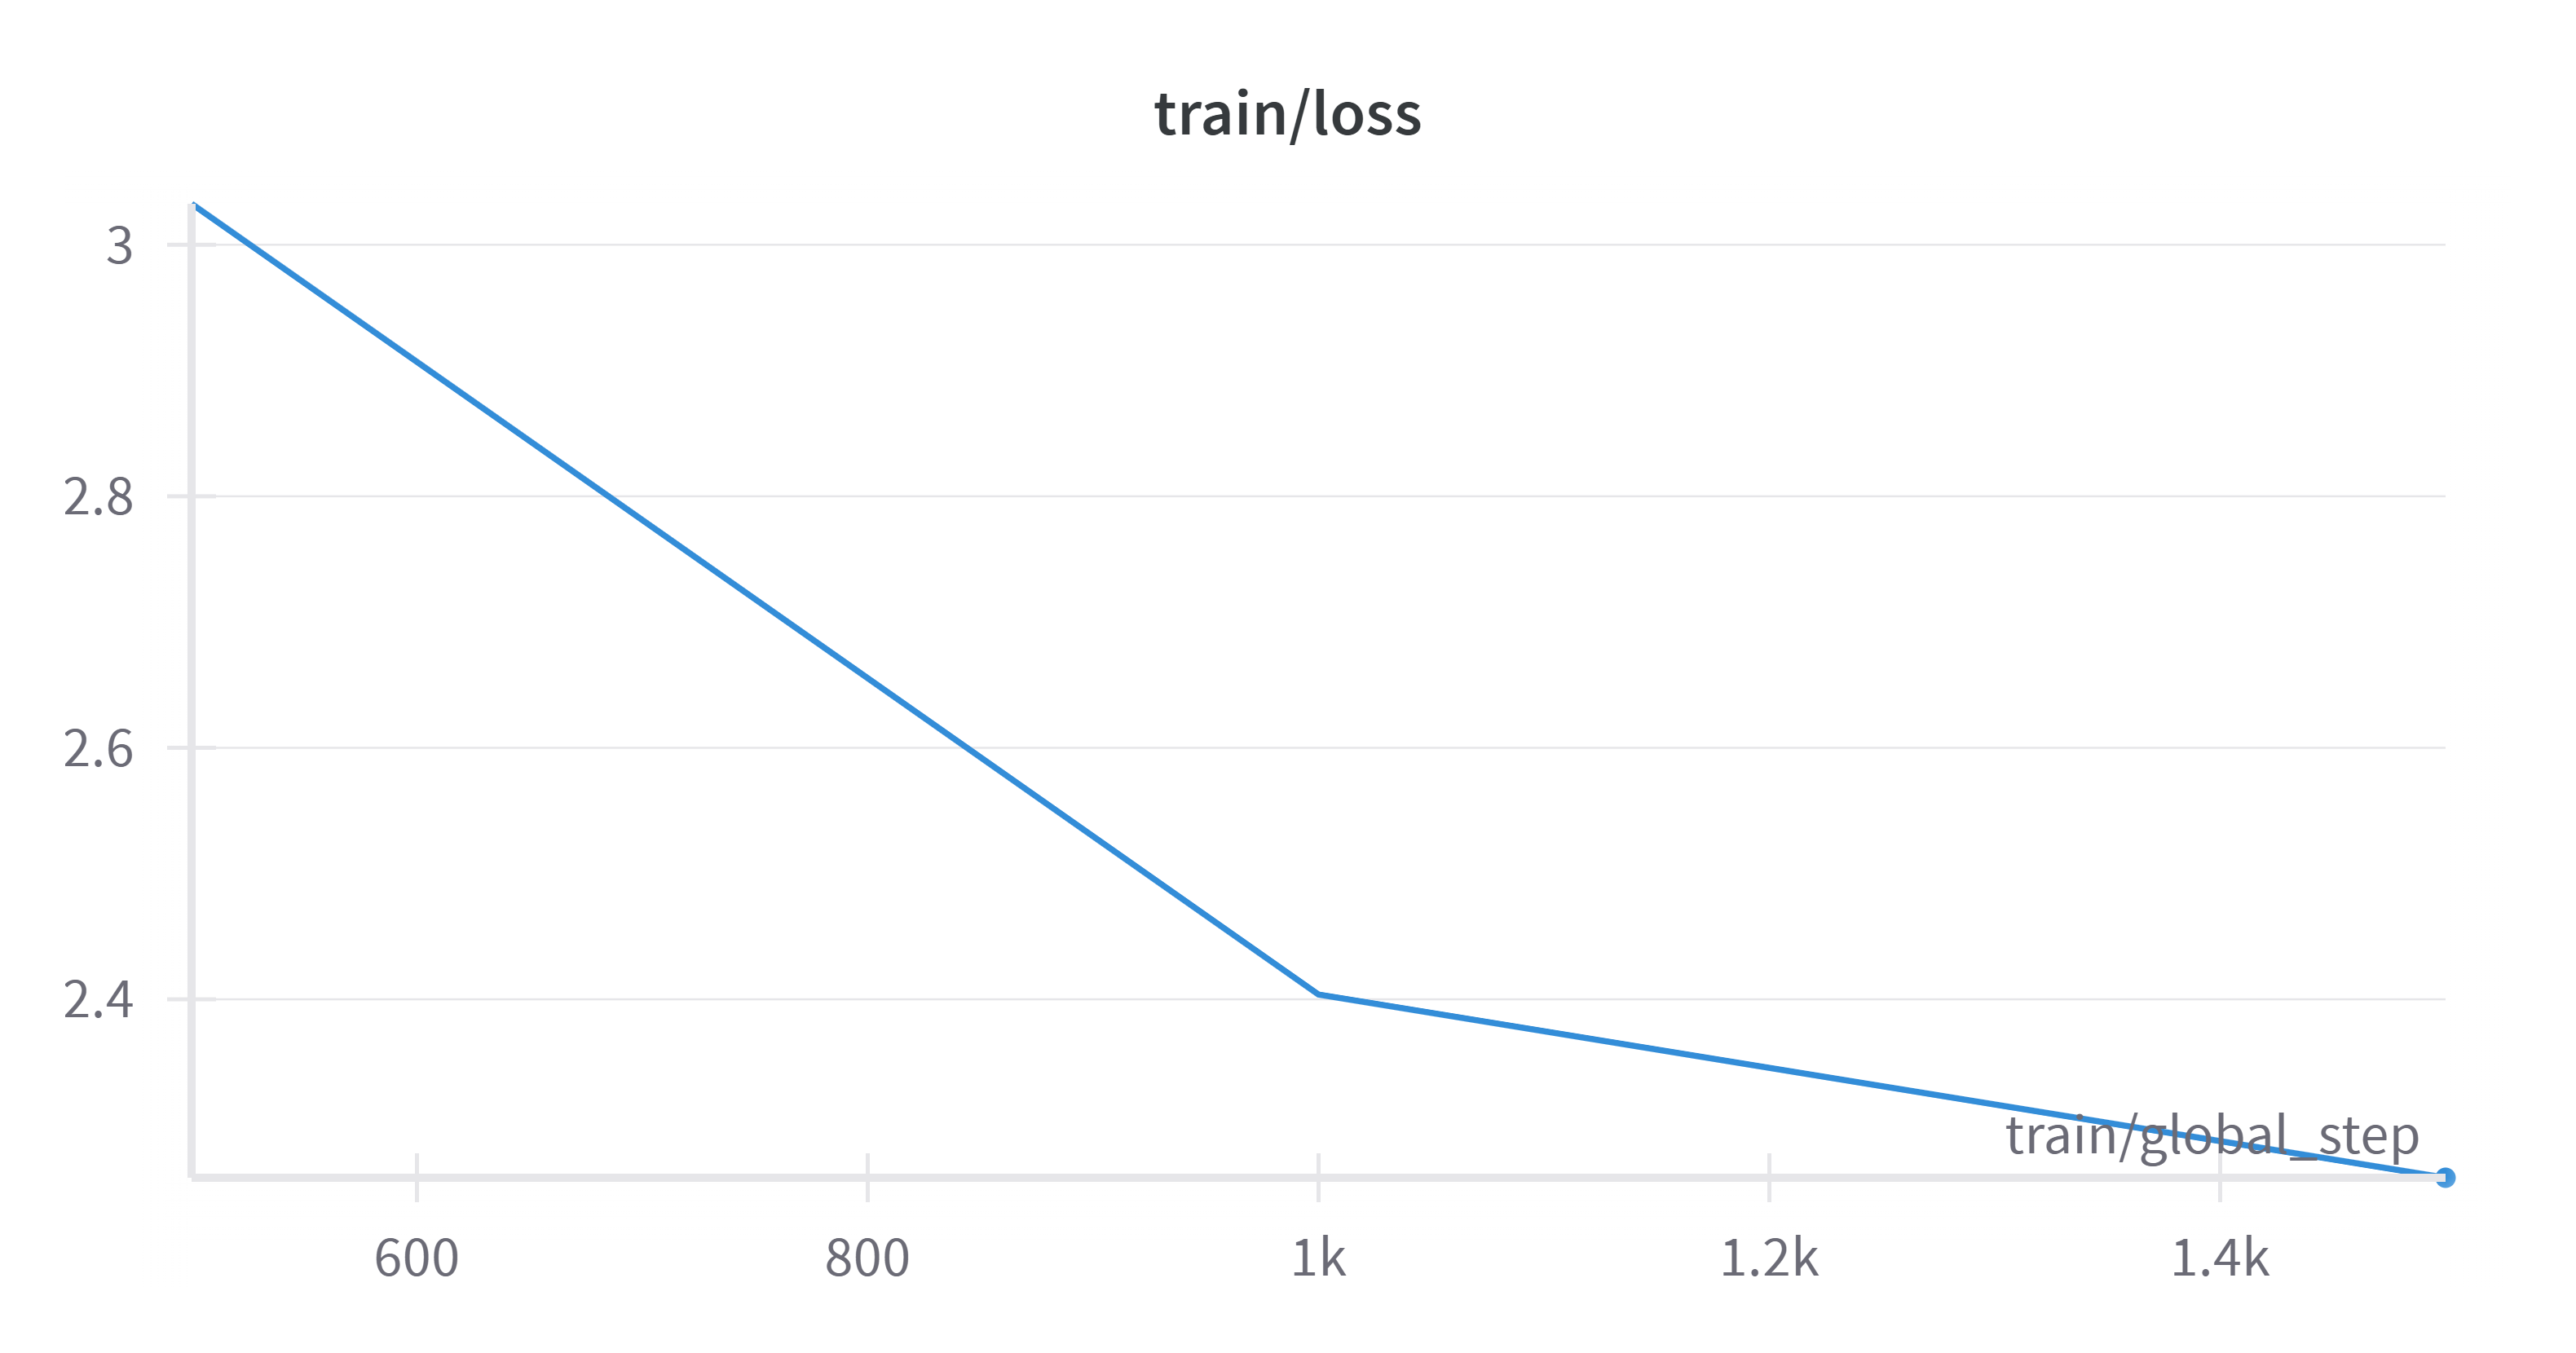
\includegraphics[width=\textwidth]{sbert_finetuned_hard_negatives.png}
\caption{Full FT (Hard): Rapid initial loss reduction followed by convergence challenges}
\end{subfigure}
\caption{Training loss curves revealing convergence patterns across different fine-tuning approaches and negative sampling strategies.}
\label{fig:training_curves_thesis}
\end{figure*}

\subsection{Training Convergence Metrics}

Table~\ref{tab:training_metrics_thesis} presents quantitative training convergence metrics including final training loss and cosine similarity accuracy.

\begin{table}[h]
\centering
\caption{Training Convergence Metrics}
\label{tab:training_metrics_thesis}
\begin{tabular}{lcc}
\toprule
Model & Final Train Loss & Eval Cosine Accuracy \\
\midrule
Full FT (Random) & 0.79 & 0.97 \\
LoRA FT (Random) & 1.42 & 0.95 \\
Full FT (Hard) & 2.26 & 0.84 \\
LoRA FT (Hard) & 3.10 & 0.78 \\
\bottomrule
\end{tabular}
\end{table}

\subsection{Training Dynamics Insights}

Combined analysis of training dynamics, loss curves, and convergence metrics reveals the true nature of fine-tuning failure:

\begin{itemize}
\item \textbf{Optimization Success vs. Performance:} Better training convergence among fine-tuned models correlates with better downstream performance, but all variants consistently underperform the base model
\item \textbf{Hard Negatives Impact:} Hard negatives cause training instability and higher final losses across both fine-tuning approaches
\item \textbf{LoRA Sensitivity:} LoRA shows greater sensitivity to negative sampling strategy, with particularly poor performance on hard negatives
\end{itemize}

\section{Comparative Analysis and Discussion}

\subsection{Cross-Method Performance Comparison}

When comparing across fine-tuning methods:

\begin{itemize}
\item \textbf{Full fine-tuning} consistently outperforms LoRA across both negative sampling strategies
\item \textbf{Random negatives} uniformly outperform hard negatives across both fine-tuning approaches
\item \textbf{Performance degradation severity} follows the pattern: LoRA Hard (-32.3\%) > Full Hard (-16.2\%) > LoRA Random (-15.5\%) > Full Random (-13.5\%)
\end{itemize}

\subsection{The Scale Disparity Effect}

The consistent underperformance across all variants strongly suggests that the fundamental issue lies in scale disparity rather than methodological choices. The base model's exposure to 9.1M MS MARCO samples during billion-scale pre-training creates an optimization landscape that cannot be meaningfully improved through 1M-sample fine-tuning.

\subsection{Embedding Space as Diagnostic Tool}

The strong correlation between embedding space degradation (visualized through UMAP) and performance degradation (measured through MRR) validates our diagnostic methodology. This correlation suggests that embedding space analysis should become standard practice in fine-tuning research, particularly when working with pre-optimized models.

\section{Validation of Hypotheses}

\section{Synthesis and Interpretation}

Our investigation reveals that all fine-tuning approaches underperformed the base model, providing evidence of fine-tuning limitations on saturated benchmarks. Hard negatives consistently harmed performance more than random negatives, revealing a paradox when applied to extensively pre-trained models. UMAP visualizations demonstrate progressive degradation from structured semantic organization to uniform distributions, with geometric changes correlating with performance degradation. LoRA models exhibited 2× slower inference despite parameter efficiency, revealing hidden computational costs.

These results suggest researchers must consider pre-training exposure when evaluating fine-tuning effectiveness, adopt embedding space analysis alongside traditional metrics, and recognize that parameter efficiency does not guarantee computational efficiency in deployment.
